\chapter{Конструкторский раздел}

% \section{Функциональная схема организации конференции}

%На рисунке \ref{img:idef0} представлена функциональная схема организации конференции в нотации IDEF0.

%\includeimage
%    {idef0}
%    {f}
%    {H}
%    {\linewidth}
%    {Функциональная схема организации конференции в нотации IDEF0}

\section{Функциональные требования к протоколу}

Ниже перечислены функциональные требования к разрабатываемому протоколу.

\begin{enumerate}
    \item Протокол должен поддерживать проведение одной конференции для произвольного количества участников.
    \item Участники должны иметь возможность подключаться и отключаться от конференции во время ее проведения.
\end{enumerate}

% \section{Граф переходов состояний для конференции}

% Конференция существует пока в ней есть хотя бы один участник.

% Конференция может находиться в следующих состояниях:

% \begin{enumerate}
%     \item Удалена или еще не создана.
%     \item Подготовительное.
%     \item Активное.
% \end{enumerate}

% В подготовительном состоянии происходит определение ролей всех участников, а также подготовка каналов передачи данных. При отключении одного из участников или подключении нового участника конференция также переходит в данное состояние.

\section{Роли участников конференции}

При создании конференции участник, который ее создает (и отправляет приглашения остальным участникам) назначается управляющим конференцией.

Управляющий конференцией имеет возможность редактировать параметры конференции, рассылать приглашения, а также передать свои полномочия другому участнику конференции.

% \section{Граф переходов состояний для участника конференции}

% 1. Не подключен к конференции.
% 2. Ожидание подключения к конференции.
% 3. Подготовительное состояние.
% 4. Активное состояние.

% Для того, чтобы подключиться к конференции, участник должен ожидать приглашения от управляющего конференцией, или от любого участника конференции (зависит от параметров самой конференции).

\section{Типы сообщений}

Разрабатываемый протокол предусматривает следующие типы передаваемых сообщений:
\begin{itemize}[label=---]
    \item \texttt{INVITE} --- приглашение в конференцию. Получатель сообщения подключается к конференции, в которой участвует отправитель.
    \item \texttt{INVITE\_ACCEPT} --- участник принимает приглашение.
    \item \texttt{INVITE\_REJECT} --- участник отклоняет приглашение.
    \item \texttt{PART\_PRESENCE} --- подключение/отключение участников конференции.
    \item \texttt{PART\_INFO} --- изменение состояния отдельного участника конференции.
    \item \texttt{REENTER} --- отправитель намеревается подключиться к существующей конференции (после потери соединения).
    \item \texttt{LEAVE} --- отправитель намеривается покинуть конференцию. Получатели должны финализировать все ресурсы, связанные с этим участником и разорвать соединения. Без использования данного типа сообщения будет происходить ожидание переподключения участника.
    \item \texttt{AUDIO} --- сообщение с аудио пакетом.
    \item \texttt{VIDEO} --- сообщение с видео пакетом.
\end{itemize}

Схема типов сообщений представлена на рисунке \ref{img:msg-types}.
\begin{figure}[h!]
  \centering
  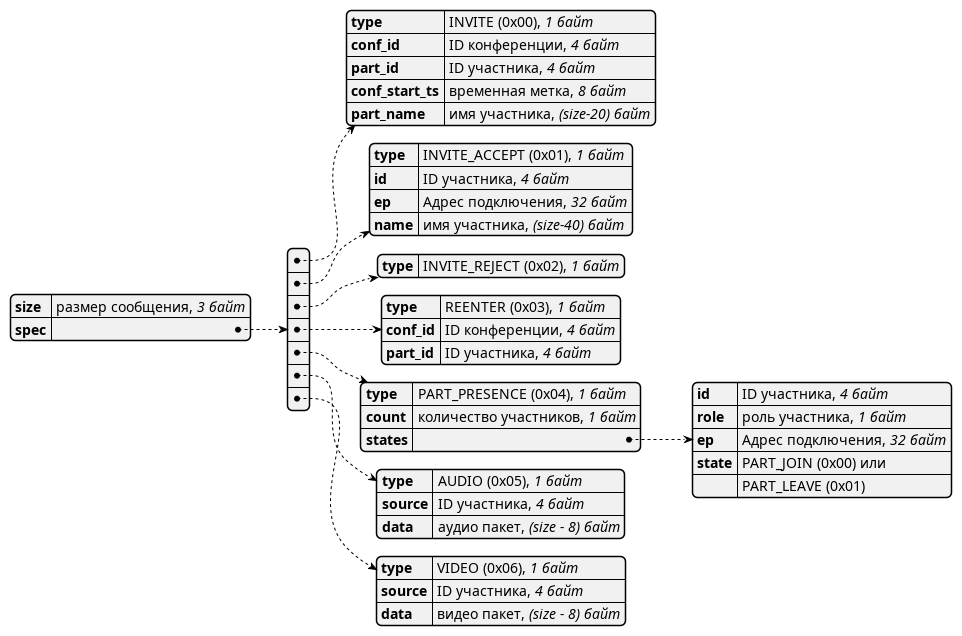
\includegraphics[width=\linewidth]{inc/diag/msg-types/msg-types.png}
  \caption{Схема типов сообщений с полями}
  \label{img:msg-types}
\end{figure}

\section{Медиа форматы}

Снижение объемов передачи аудио/видео данных по сети требует использования кодеков, сжимающих медиа данные. Для разрабатываемого протокола применяются кодеки AAC \cite{aac} и H.264 \cite{h264}. Аудио кадр кодируется в стерео формате с частотой 48кГц. Видео кадр кодируется в разрешении 320 на 180 пикселей и частотой в 30 кадров в секунду.

\section{Взаимодействия сторон}

Рассмотрим сценарий с двумя участниками --- <<А>> и <<Б>>. Для организации конференции, участник <<А>> отправляет участнику <<Б>> сообщение типа \texttt{INVITE}.
После чего участник <<Б>> должен ответить на него сообщением \texttt{INVITE\_ACCEPT} для подключения к конференции участника <<А>>.
После успешного подключения, происходит инициализация каналов передачи медиа данных. Аудио и видео пакеты передаются с использованием сообщений типов \texttt{AUDIO} / \texttt{VIDEO}.
Диаграмма последовательности описанного процесса представлена на рисунке \ref{img:conf-2}.

\begin{figure}[H]
  \centering
  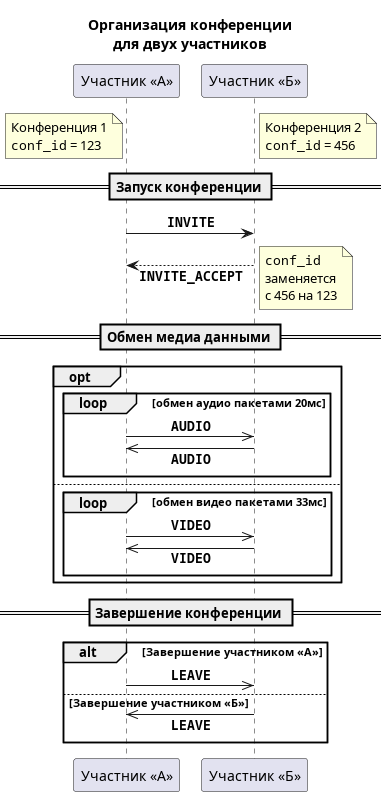
\includegraphics[width=0.6\linewidth]{inc/diag/seq-2/conf-2.png}
  \caption{Диаграмма последовательности для организации конференции для двух участников}
  \label{img:conf-2}
\end{figure}

Подключение последующих участников происходит аналогичным образом --- один из активных участников конференции отправляет сообщение с приглашением в конференцию новому участнику, и, после получения ответного сообщения \texttt{INVITE\_ACCEPT}, отправляет сообщение \texttt{PART\_PRESENCE} остальным участникам конференции для уведомления о подключении нового участника.
Каждый из остальных участников, получив сообщение \texttt{PART\_PRESENCE} отправляет приглашение \texttt{INVITE} новому участнику для инициализации каналов связи между всеми парами участников конференции.
Диаграмма последовательности описанного процесса представлена на рисунке \ref{img:conf-3}.

\begin{figure}[H]
  \centering
  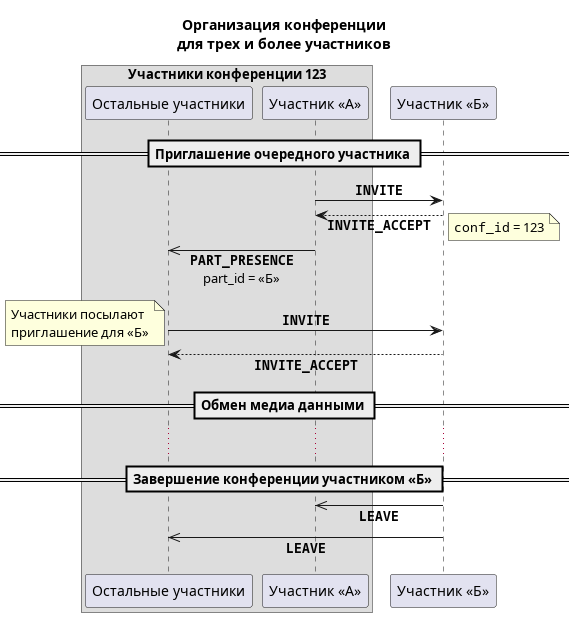
\includegraphics[width=0.9\linewidth]{inc/diag/seq-3/conf-3.png}
  \caption{Диаграмма последовательности для организации конференции для трех и более участников}
  \label{img:conf-3}
\end{figure}

\section{Шифрование}

Шифрование используется для обеспечения целостности и конфиденциальности передаваемых данных. (Защита от подслушивания, порчи и/или подделки сообщений).
Проверка сертификатов разрабатываемым протоколом не предусмотрена, но может быть проведена при повторном соединении с участником.
В качестве протокола шифрования используется TLS v1.3 \cite{tls}.

% TODO: Обоснованность использования TCP вместо RTC и UDP --- TLS не работает поверх UDP?

Выбор между протоколами TCP+TLS и SRTP для организации бессерверных видео конференций зависит от ряда факторов и требований. Рассмотрим преимущества и недостатки каждого из подходов:

Преимущества использования TCP+TLS:

\begin{itemize}[label=---]
  \item Надежность и безопасность --- TCP обеспечивает надежную доставку данных, а TLS предоставляет шифрование и аутентификацию, защищая передаваемые данные.
  \item Совместимость --- TCP и TLS являются широко распространенными и поддерживаемыми протоколами, что упрощает интеграцию с различными системами и платформами.
  \item Развитая инфраструктура --- для TCP+TLS существует большое количество инструментов, библиотек и готовых решений, упрощающих разработку.
  %\item Поддержка NAT и фаерволов --- TCP способен работать через NAT-устройства и фаерволы, что важно для организации бессерверных конференций.
\end{itemize}

Недостатки:

\begin{itemize}[label=---]
  \item Более высокая задержка --- TCP имеет больше накладных расходов по сравнению с UDP-протоколами, что может повлиять на качество аудио и видео.
  \item Более высокие требования к ресурсам --- TCP-стек требует больше памяти и вычислительных ресурсов, что может быть критично для устройств с ограниченными возможностями.
\end{itemize}

Преимущества использования SRTP:

\begin{itemize}[label=---]
  \item Низкая задержка --- SRTP, построенный поверх UDP, имеет меньше накладных расходов, что позволяет обеспечить более высокое качество аудио и видео.
  \item Меньшее потребление ресурсов --- SRTP более эффективен в плане использования памяти и вычислительной мощности, что важно для мобильных устройств.
  \item Специализация на мультимедиа --- SRTP разработан специально для защищенной передачи аудио и видео данных, в отличие от более универсального TCP+TLS.
\end{itemize}
  
Недостатки:

\begin{itemize}[label=---]
  \item Ограниченная совместимость --- SRTP не так широко распространен, как TCP+TLS, что может усложнить интеграцию с существующими системами.
  \item Меньшая надежность --- UDP, лежащий в основе SRTP, не гарантирует доставку данных, что может привести к потере пакетов в неблагоприятных сетевых условиях.
  \item Сложность реализации --- SRTP требует реализации дополнительных механизмов для управления ключами шифрования, что усложняет разработку.
\end{itemize}

%В итоге, выбор между TCP+TLS и SRTP зависит от конкретных требований проекта. TCP+TLS лучше подходит для приложений, где важны надежность, безопасность и совместимость, в то время как SRTP более эффективен для передачи мультимедийных данных с низкой задержкой. Важно также учитывать ресурсные ограничения целевых платформ и сложность реализации каждого из подходов.

\section{Переподключение}

При потере соединения без получения сообщения \texttt{LEAVE} небходимо ожидать переподключение участника в течении 30 секунд. Если участник так и не подключился к конференции, то он считается вышедшим из конференции и в последующем сможет подключиться к ней только через приглашение от другого участника конференции.

Переподключение производится отправкой сообщения \texttt{REENTER} с идентификатором текущей конференции и идентификатором участника, потерявшего соединение. Если сообщение было получено по истечению 30 секундного интервала --- оно отбрасывается, соединение закрывается и участник считывается неподключившимся.

\section{Определение качества каналов связи}

Для реформирования топологии связей в бессерверных видео конференциях необходимо определить качество существующих каналов связи между участниками. Это может быть выполнено с использованием метрик, которые зависят от следующих параметров: временные метки отправки/приема аудио/видео пакета; размер пакета в байтах; количество переданных и повторно переданных пакетов.

На основе этих параметров могут быть вычислены такие показатели качества как:
\begin{itemize}[label=---]
  \item задержка передачи --- временная разница между отправкой и получением пакета;
  \item джиттер --- вариация задержки между последовательными пакетами;
  \item пропускная способность --- объем данных, переданных за определенный период времени.
\end{itemize}

Используя данные метрики, можно оценить состояние каналов связи между участниками конференции и принять решение о необходимости реформирования топологии. Например, если канал между двумя участниками характеризуется высокой задержкой и потерями пакетов, можно рассмотреть вариант передачи медиа данных через третьего участника, который имеет более качественное соединение. Это позволит сократить нагрузку на перегруженный канал и переложить часть вычислительной нагрузки по перекодированию на более мощный клиент.
